\documentclass[conference]{IEEEtran}
% packages
\usepackage{xspace}
\usepackage{hyperref}
\usepackage{todonotes}
\usepackage{tikz}
\usepackage[utf8]{inputenc}

%  commands
% \newcommand{\todo}[1]{$\langle\!\langle$\marginpar[\raggedleft$\triangleright\triangleright\triangleright$]{$\triangleleft\triangleleft\triangleleft$}\textsf{#1}$\rangle\!\rangle$}
\def\CC{{C\nolinebreak[4]\hspace{-.05em}\raisebox{.4ex}{\tiny\bf ++}}}
\def\ea{\,et\,al.\ }

\begin{document}
	
% paper title
\title{Riss Solver Framework v5.05}

% author names and affiliations
% use a multiple column layout for up to three different
% affiliations
\author{
\IEEEauthorblockN{Lucas Kahlert, Franziska Krüger, Norbert Manthey and Aaron Stephan}
\IEEEauthorblockA{Knowledge Representation and Reasoning Group\\TU Dresden, Germany}
}

\maketitle

\def\coprocessor{\textsc{Coprocessor}\xspace}
\def\glucose{\textsc{Glucose~2.2}\xspace}
\def\minisat{\textsc{Minisat~2.2}\xspace}
\def\riss{\textsc{Riss}\xspace}
\def\priss{\textsc{Priss}\xspace}
\def\pcasso{\textsc{Pcasso}\xspace}

% the abstract is optional
\begin{abstract}
The sequential SAT solver \riss combines the Minisat-style solving engine of \glucose with a state-of-the-art preprocessor \textsc{Coprocessor} and adds many modifications to the search process. 
\riss allows to use inprocessing based on \coprocessor.
Based on this \riss, we create a parallel portfolio solver \priss, which allows clause sharing among the incarnations, as well as sharing information about equivalent literals. 
Finally, the search space partitioning SAT solver \pcasso is built on top of \priss, allowing to solve a formula with a portfolio solver, and additionally solve this formula with iterative partitioning where each partition is solved with the portfolio solver \priss, including clause sharing over partitions. 
\end{abstract}

\section{Introduction}

The CDCL solver \riss was first build on the \textsc{Minisat} search engine~\cite{EenS:2003}, and next incorporated the improvements that have been proposed for \glucose ~\cite{AudemardS:2009,Audemard:2012:RRS:2405292.2405308}. 
Afterwards, more search algorithm extensions have been added, and \riss is equipped with the preprocessor \textsc{Coprocessor}~\cite{Manthey:2012}, 
that implements most of the recently published formula simplification techniques, ready to be used as inprocessing as well by taking care of learned clauses. 
The parallel simplification techniques of \coprocessor are disables in the used configurations. 
The aim of the solver is to provide a huge set of options on the one hand, to be able to adapt to new SAT applications, and an efficient implementation on the other hand. 
Due to the huge configuration space, to increase robustness an algorithm for checking the reported satisfying assignment, as well as an on-the-fly DRAT proof verification are added to the sequential solver -- as the combination of all parameter configurations cannot be tested extensively. 

Similarly, we build the parallel solver \priss and \pcasso, which again are highly configurable. 
In \priss, each incarnation of \riss can be configured, and furthermore the properties of information sharing can be set. 
\priss first runs a global formula simplification step, before search is started in parallel. 
Each solver incarnation can simplify the formula again, where currently only equivalence preserving techniques are enabled. 
An incarnation can also work on the original formula. 

Finally, \pcasso can \riss or \priss as base solver. 
\pcasso solves a formula based on iterative partitioning. 
Furthermore, an additional \priss incarnation is added to solve the given formula. 
Similarly to the other two solvers, \pcasso first simplifies the formula with a \coprocessor incarnation before starting parallel search.

The incremental solver interface is currently only supported by \riss. 
\priss supports a similar interface, and can be used to use a parallel portfolio solver as incremental solver. 

The remainder of the document describes only the changes that have been applied to the tools compared to their previous versions of 2014~\cite{Mriss427-2014,MRissBlackbox-2014,pcasso2014}.

\section{Modifications of Riss and Coprocessor}

\textsc{Riss 5.05} is an extension of \textsc{Riss 4.27}, where a few techniques have been removed to clean the code base, which has been executed during search. 
On the other hand, many modification have been added, among others ideas that have been proposed in recent \textsc{Minisat}-Hack-Tracks. 
The considered extensions come from the solvers \textsc{RestartSAT}, \textsc{CirMiniSAT}, \textsc{MinitSAT}, \textsc{mipisat} and \textsc{MiniSat\_HACK\_999ED}. 
All novel features are turned off by default, such that the default behavior of the solver does not change too much when modifying the implementation. 
The initialization of the solver has been improved: the activities for decision variables are initialized with decreasing values. 

\subsection{Conflict Analysis and Minimization}

Compared to \glucose, the LBD of the currently constructed learnt clause is only re-calculated if a minimization technique modified the clause.
Finally, \riss implements a modified variables on \emph{restricted extended-resolution}~\cite{DBLP:conf/aaai/AudemardKS10,MextendedResolutionInModernSAT}. 
This variant also allows to structurally extract binary AND-gates from the formula, to later use this information to reduce learned clauses by replacing both input literals with the output literal of such a gate. 
Finally, another unpublished additional clause minimization technique is added to conflict analysis. 
Removing learnt clauses can be done as in \glucose based on the LBD of the clause, and an dynamic schedule. 
However, the clause activity based version and the more static schedule of \minisat are also supported, including the ideas of the randomly assigned activity from~\cite{DBLP:journals/corr/JabbourLSS14}. 

\subsection{Unit Propagation}

The implementation of unit propagation has also been improved: 
Instead of storing binary clauses in an extra watch list, as implemented in \glucose, we store all clauses in a common watch list. 
However, each list entry stores a Boolean flag which indicated whether the current clause is binary, such that we just have to work with the \emph{blocking literal}, and do not need to access the actual clause. 
By using only one watch list, the used memory can be reduced compared to \glucose.

\subsection{Coprocessor}

\coprocessor received only little attention. 
Small changes have been applied to the execution order of the simplification techniques, which now all process least occurring literals first (except \emph{bounded variable addition}~\cite{Mbva}). 
Furthermore, \coprocessor now runs all activated simplification techniques twice in the specified order. 

We added an implementation of an elimination routine to remove \emph{resolution asymmetric tautologies} (RAT)~\cite{inprocessingRules}. 
Based on this routine, and the idea of \emph{covered literal elimination}~\cite{MclePPdrat}\footnote{Developped independly also by Heule et al.}, we implemented routines to add a redundant clause, if it subsumes another clause that is present in the formula. 
Hence, \coprocessor allows to perform \emph{vivification} by adding \emph{asymmetric tautologies} that subsume other clauses. 
Similarly, \coprocessor can add \emph{blocked clauses}, \emph{covered clauses}, or \emph{RATs}. 

The implemented extraction of XORs in the formula does not use a detection based on subsumption due to its high time consumption. 
On the other hand, the XOR reasoning does not only use information about retrieved unit clauses and equivalent literals, but furthermore encodes ternary XORs back into CNF. 

\section{The Parallel Portfolio Solver Priss}

The parallel portfolio solver \priss can simplify the formula with \coprocessor for all its incarnations in parallel. 
Afterwards, each incarnation can work on this formula, such that information sharing is easier -- all clauses can be shared as long as no further simplification that do not preserve equivalence are applied. 
An incarnation can choose to to work on the original formula instead, but then (currently) knowledge sharing with this incarnation is disabled. 

\subsection{Information Sharing}

Incarnations of \riss in \priss can share learned clauses, as well as information about equivalent literals. 
\priss has two storages that are implemented as ring buffer. 
The first buffer stored unit clauses and equivalent literal classes. 
The other buffer stores shared learned clauses. 
Information is received whenever an incarnation should do a search decision for decision level 1. 
Due to the ring buffer implementation, incarnations might miss shared clauses. 
On the other hand, this implementation ensures that the size of the shared buffer is limited. 

Received clauses can be minimized by \emph{vivification} and reduced clauses can be shared immediately, as proposed in~\cite{DBLP:conf/sat/WieringaH13}. 
Learned clauses are shared after (i) they have been learned, (ii) they have been used in unit propagation~\cite{glucose4sharing}, or (iii) after they have been used for conflict analysis again. 
This way, only ``relevant'' learned clauses are shared. 

Before a clause is shared, it has to pass a size filter and an LBD filter. 
These filters can be set to static thresholds. 
However, the thresholds can also be increased dynamically, if not enough clauses are sent. 
Finally, in case not all clauses are selected for sharing (the above (ii) and (iii)), then the filters might not be used, as the clauses turned out to be relevant for the current incarnation already. 

The activity of received clauses is set to the value of the most recently learnt clause. 
The LBD of the received clause is estimated based on the size to LBD ratio of the current incarnation, as on search level $0$ there are not variable assignments and levels that can be used to determine the actual LBD of the clause. 
Furthermore, received clauses are ignored in the next removal iteration. 
All these options can be specified for each incarnation -- in the submitted version the parameters are fixed as described above. 

\subsection{Configuration Selection}

For each incarnation in the portfolio, the configuration can be specified on the command line. 
In the the used preset, the first three configurations are the most robust configurations that have been while working with application formulas. 
The simplification of the first incarnation is used for the full portfolio and the other two incarnations do not participate in information sharing. 
The first incarnation only sends information, but does not receive information. 
The remaining configurations are based on configurations that showed good performance and are extended with randomization, such that the portfolio works better especially on satisfiable formulas. 
Furthermore, \emph{inprocessing} with equivalence preserving techniques is enabled, including replacing equivalent literals. 

\section{The Search Space Partitioning Solver Pcasso}

\pcasso implements solving formulas in parallel based on iterative search space partitioning~\cite{Miterative-splitting}. 
The partitioning is the same as in last years version. 

\subsection{Solving In Parallel}

Besides the iterative partitioning approach, a \priss incarnation is executed in parallel. 
This incarnation is also used for the initial formula simplification. 
Furthermore, shared information is forwarded to the partitioning approach. 

\subsection{Solving Partitions}

Compared to last years version the solver that solved the partitions is exchanged. 
Instead of \textsc{Glucose 2.2}, we now use either a \riss or a \priss incarnation. 
Due to the possibility of inprocessing, upward clause sharing in the partition tree is currently disabled. 
Learned information are still shared downward in the tree. 
With the \priss incarnation, a partition can also be solved with a parallel solver. 
Then, the incarnations in \priss share their learned information with the other internal incarnations, as well as with their child partitions.

\section{Incremental SAT Solving with Riss}

\riss implements the ipasir interface. 
\riss furthermore implements a similar C interface, where a configuration can be selected. 
The ipasir interface is a wrapper for the internal interface. 

\coprocessor also provides an incremental interface, where formula simplification can be applied to a formula.

\section{Special Algorithms, Data Structures, and Other Features}

Due to the high number of parameters \riss implements a configuration prediction. 

\subsection{Black Box}

The machine learning front end is based on the feature extraction routines implemented in \riss~\cite{Mblackbox}. 
Compared to last years version we improved the implementation of the extraction to reduce the memory consumption considerably by consuming slightly more run time. 

The Knowledge base for prediction is now integrated into the solver, such that there are no dependencies to external tools any longer. 
From a formula we extract 382 features, which are projected to 40 values by \emph{principal component analysis} (PCA). 
We replaced the selection based on \emph{information gain ratio}, as in the latter case the projected values still correlate. 
After PCA there is no more correlation among the values. 
Based on the data base, which is created based on 14 configurations and 2200 application formulas. 
The best prediction we found so this set uses a k-nearest neighbor with only a single neighbor, instead of the random decision forest we in \textsc{Riss 4.27 BlackBox}.  
This might be the case due to the small number of formulas and the comparably high number of configurations. 
We currently experiment how to improve this prediction, especially for working better on unknown formulas. 

The implementation of PCA is based on two external libraries: \emph{Libpca}\footnote{\url{http://sourceforge.net/projects/libpca/}} and \emph{armadillo}\footnote{\url{http://arma.sourceforge.net/}}.

% \begin{figure*}[t!!]
% \centering
% 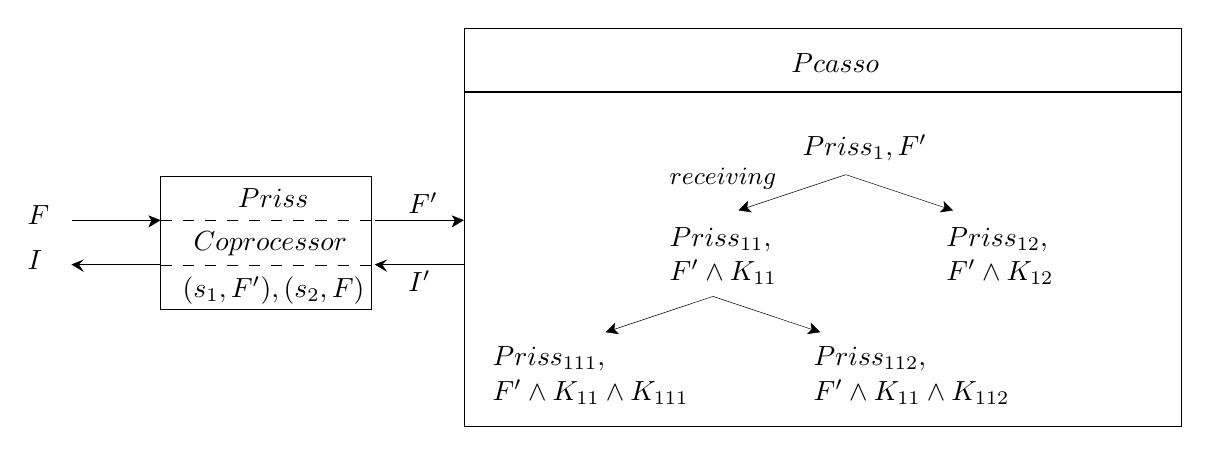
\begin{tikzpicture}[y=0.80pt, x=0.80pt, yscale=-1.000000, xscale=1.000000, inner sep=0pt, outer sep=0pt]

  \path[draw=black,line width=0.160pt,rounded corners=0.0000cm] (370,-453) rectangle (465,-393);
  \path[draw=black,dash pattern=on 4.00pt,line width=0.160pt]   (370,-433)  -- (465,-433);
  \path[draw=black,dash pattern=on 4.00pt,line width=0.160pt]   (370,-413)  -- (465,-413);
  \path[fill=black] (405,-439) node[above right] (text4428) {$Priss$};
  \path[fill=black] (385,-417) node[above right] (text4432) {$Coprocessor$};
  \path[fill=black] (380,-395) node[above right] (text4446) {$(s_1, F'), (s_2, F)$};

  % output arrow
  \begin{scope}[shift={(-130,6.89156)}]
    \path[draw=black,line width=0.160pt] (463,-420) -- (500,-420);
    \path[fill=black] (465,-417) -- (460,-420) -- (465,-422) -- (463,-420) -- cycle;
    \path[draw=black,line width=0.160pt] (465,-417) -- (460,-420) -- (465,-422) -- (463,-420) -- cycle;
  \end{scope}

  % input arrow
  \begin{scope}[shift={(-10,6.89156)}]
    \path[draw=black,line width=0.160pt] (340,-440) -- (376.0260,-440);
    \path[fill=black] (374.7760,-442) -- (379.7760,-440) -- (374.7760,-437) -- (376.0260,-440) -- cycle;
    \path[draw=black,line width=0.160pt] (374.7760,-442) -- (379.7760,-440) -- (374.7760,-437) -- (376.0260,-440) -- cycle;
  \end{scope}

  \path[fill=black] (310,-431) node[above right] (text4466) {$F$};
  \path[fill=black] (310,-411) node[above right] (text4470) {$I$};

  % intermidiate output arrow
  \begin{scope}[shift={(7,6.89156)}]
    \path[draw=black,line width=0.160pt] (463,-420) -- (500,-420);
    \path[fill=black] (465,-417) -- (460,-420) -- (465,-422) -- (463,-420) -- cycle;
    \path[draw=black,line width=0.160pt] (465,-417) -- (460,-420) -- (465,-422) -- (463,-420) -- cycle;
  \end{scope}

  % intermidiate input arrow
  \begin{scope}[shift={(7,6.89156)}]
    \path[draw=black,line width=0.160pt] (460,-440) -- (496.0260,-440);
    \path[fill=black] (494.7760,-442) -- (499.7760,-440) -- (494.7760,-437) -- (496.0260,-440) -- cycle;
    \path[draw=black,line width=0.160pt] (494.7760,-442) -- (499.7760,-440) -- (494.7760,-437) -- (496.0260,-440) -- cycle;
  \end{scope}

  \path[fill=black] (482,-436) node[above right] (text4502) {$F'$};
  \path[fill=black] (482,-401) node[above right] (text4506) {$I'$};

  \path[draw=black,line width=0.160pt,rounded corners=0cm] (507,-520) rectangle (831,-340);

  \path[fill=black] (655,-500) node[above right] (text4498) {$Pcasso$};
  \path[draw=black,line join=miter,line cap=butt,miter limit=4.00,line width=0.435pt] (507,-491) -- (831,-491);

  % level one
  \path[fill=black] (660,-460) node[above right] (text4510) {$Priss_1,  F'$};

  \path[fill=black] (600,-447) node[above right] (text4511) {\small$receiving$};

  % level two
  \begin{scope}[cm={{0.94861,-0.31644,0.31644,0.94861,(255.76474,179.04113)}}]
    \path[draw=black,line width=0.183pt] (555.1339,-466.1446) -- (602.1395,-466.1446);
    \path[shift={(91.12944,-46.14463)},fill=black] (465.2240,-417.5000) -- (460.2240,-420.0000) -- (465.2240,-422.5000) -- (463.9740,-420.0000) -- cycle;
    \path[shift={(91.12944,-46.14463)},draw=black,line width=0.160pt] (465.2240,-417.5000) -- (460.2240,-420.0000) -- (465.2240,-422.5000) -- (463.9740,-420.0000) -- cycle;
  \end{scope}

  \begin{scope}[cm={{-0.94861,-0.31644,-0.31644,0.94861,(1103.2911,179.04114)}}]
    \path[draw=black,line width=0.183pt] (555.1339,-466.1446) -- (602.1395,-466.1446);
    \path[shift={(91.12944,-46.14463)},fill=black] (465.2240,-422.5000) -- (463.9740,-420.0000) -- (465.2240,-417.5000) -- (460.2240,-420.0000) -- cycle;
    \path[shift={(91.12944,-46.14463)},draw=black,line width=0.160pt] (465.2240,-422.5000) -- (463.9740,-420.0000) -- (465.2240,-417.5000) -- (460.2240,-420.0000) -- cycle;
  \end{scope}

  \path[fill=black] (600,-419) node[above right] (text4518) {$Priss_{11},$};
  \path[fill=black] (600,-404) node[above right] (text4519) {$F' \land K_{11}$};
  
  \path[fill=black] (725,-419) node[above right] (text4522) {$Priss_{12},$};
  \path[fill=black] (725,-404) node[above right] (text4523) {$F' \land K_{12}$};


  % level three

  \begin{scope}[shift={(-60,55)},cm={{0.94861,-0.31644,0.31644,0.94861,(255.76474,179.04113)}}]
    \path[draw=black,line width=0.183pt] (555.1339,-466.1446) -- (602.1395,-466.1446);
    \path[shift={(91.12944,-46.14463)},fill=black] (465.2240,-417.5000) -- (460.2240,-420.0000) -- (465.2240,-422.5000) -- (463.9740,-420.0000) -- cycle;
    \path[shift={(91.12944,-46.14463)},draw=black,line width=0.160pt] (465.2240,-417.5000) -- (460.2240,-420.0000) -- (465.2240,-422.5000) -- (463.9740,-420.0000) -- cycle;
  \end{scope}

  \begin{scope}[shift={(-60,55)},cm={{-0.94861,-0.31644,-0.31644,0.94861,(1103.2911,179.04114)}}]
    \path[draw=black,line width=0.183pt] (555.1339,-466.1446) -- (602.1395,-466.1446);
    \path[shift={(91.12944,-46.14463)},fill=black] (465.2240,-422.5000) -- (463.9740,-420.0000) -- (465.2240,-417.5000) -- (460.2240,-420.0000) -- cycle;
    \path[shift={(91.12944,-46.14463)},draw=black,line width=0.160pt] (465.2240,-422.5000) -- (463.9740,-420.0000) -- (465.2240,-417.5000) -- (460.2240,-420.0000) -- cycle;
  \end{scope}

  \path[fill=black] (520,-365) node[above right] (text4530) {$Priss_{111},$};
  \path[fill=black] (520,-350) node[above right] (text4531) {$F' \land K_{11} \land K_{111}$};
  \path[fill=black] (665,-365) node[above right] (text4534) {$Priss_{112},$};
  \path[fill=black] (665,-350) node[above right] (text4535) {$F' \land K_{11} \land K_{112}$};

\end{tikzpicture}
 
% \caption{Schema of \pcasso with \priss incarnations to solve partitions recursively and a global \priss to simplify the original formula.} \label{fig:pcassoBlackbox}
% \end{figure*}

\section{SAT Race 2015 Specifics}

\riss and \coprocessor are implemented in \CC. 
All simplification techniques inside \coprocessor are implemented in separate classes to increase the structure of the code. 
\priss and \pcasso implement the parallel code for multi-core architectures with the pthreads library.

The solvers are submitted to all tracks that are offered. 
The submitted configurations are described below. 

\subsection{Sequential SAT Solving}

The submitted default configuration of \textsc{Riss 5.05} uses the following techniques:
%
bounded variable elimination, 
cardinality extraction and Fourier-Motzkin, 
five iterations of reasoning on the binary implication graph,
covered literal elimination,
detecting and replacing equivalent literals with structural hashing of AND-gates and with strongly connected components on the binary implication graph,
XOR reasoning, 
and variable renaming to compact the representation of the formula during search. 
Furthermore, the unpublished learned clause minimization is used, and the activities for decision variables is initialized as described above. 
Finally, during clause removal we keep $1$ percent of the heuristically ``worst'' learned clauses. 
The second sequential configuration uses the \emph{black box} prediction. 

\subsection{Incremental SAT Solving} \label{ss:incsolving}

The incremental versions do not use formula simplification, but instead use methods to reduce the overhead of solver calls. 
\textsc{Riss 5.04} removes satisfied clauses only if one of the first two literals is satisfied, similarly to \textsc{Glucose 3.0}. 
The simplification to remove satisfied clauses is executed only every 16 attempts. 
The variables, which are used in the assumptions are not considered to calculate the LBD of learned clauses. 
The activity of variables is bumped more compared to the usual configuration. 
Restarts are based on the matching trail restarts of \textsc{RestartSAT}. 
During a restart, \riss does not jump beyond assumptions (except every 1024th attempt). 
Finally, the counters of the solver are reset every $3$rd call to solve an updated formula. 

The incremental version of \textsc{Riss 5.05} uses the same configuration and furthermore adds initializing the variable activities as in the usual configuration. 
Furthermore, after $50000$ conflicts (dependent on counter resets), a formula simplification is triggered, which executes the same techniques as in the sequential solver configurations, except variable elimination, covered literal elimination and variable renaming. 
Instead, subsumption and self-subsuming resolution are executed, such that only equivalence preserving techniques are used and no variables are eliminated or renamed. 
After this simplification, the next simplification is allowed after another $1000000$ conflicts.


\subsection{Parallel SAT Solving}

\todo{update numbers}

In \pcasso, we use different configurations depending on the number of available computational resources. 
The configuration of \pcasso uses a global \priss incarnation with $3$ workers. 
Another $3$ workers are used for solving in the partitioning approach. 
The values are increased to $4$ workers in \priss and $8$ in partitioning. 
The full number of cores is not used, as the slowdown based on resource sharing is too high with the currently implemented data structures, as explained in~\cite{portfolioSlowdown}. 
Each node in the partition tree is allowed to store 100 learned clauses, as well as 100 groups of unit clauses or equivalent literals. 
We do not utilize hyper threads. 

The second configuration of \pcasso (BlackBox) uses the same number of workers. 
However, one configuration of \priss uses the predicted configuration. 
Furthermore, clause sharing inside the partition tree is enhanced by allowing larger ring buffers to store more clauses, namely 16000 per partition. 
The incarnations of \riss use the same inprocessing setup as the solver that is used in version $5.05$ in the incremental track (see Section~\ref{ss:incsolving}).
% This approach is visualized in Figure~\ref{fig:pcassoBlackbox}.

\section{Availability}

All tools in the solver collection are available for research. 
Besides the above mentioned tools, we furthermore provide a preliminary parallel DRAT proof verifier, as well as the model checker \textsc{ShiftBMC} in this package.
The framework can be downloaded from \url{http://tools.computational-logic.org}.

\section*{Acknowledgment}
The author would like to thank the developers of \glucose and \minisat. 
The computational resources to develop, evaluate and configure the SAT solver have been provided the ZIH of TU Dresden. 
This project is supported by the DFG grant HO 1294/11-1. 

% \bigskip
% What should not be in the system description:
% \begin{enumerate}
%   \item Basic definitions related to SAT. (However, any formal notations used in the description should be defined.)
%   \item Empirical results on the solver's performance.
% \end{enumerate}
% 
\bibliographystyle{IEEEtran}
\bibliography{local}

\end{document}



% more infos

current pcasso call (test tree communication, no parallel priss, no cross link, no priss in pcasso)

./pcasso -threads=2 -model -work-conflicts=-1 -work-timeout=-1 -split-mode=2 -split-timeout=1024 -presel-fac=0.1 -presel-min=64-presel-max=1024 -fail-lit=2 -nec-assign=2 -num-iterat=3 -con-resolv=1 -bin-const -la-heur=4 -presel-heur=2-clause-learn=2 -dir-prior=3 -child-count=7 -shrk-clause -var-eq=3-split-method=1 -split-depth=0 -dseq -h-acc=3 -h-maxcl=7 -h-cl-wg=5-h-upper=10900 -h-lower=0.1 -shpool-size=15000-shclause-size=2 -stop-children -adp-preselS=7 -sort-split -verbosity=1 -verb=1 -print-tree -g-priss-threads=0 -no-use-priss -no-crosslink -pcasso-com-config=small -g-priss-config=delta -quiet ~/cnf/safe-30-h29-unsat.cnf

current priss call: (especially the independent flag can be combined with other configuration presents to run independent solvers in parallel without communication)

./priss -threads=4 -showUnusedParam -pIncSetup=[3]-independent -addSetup -ppconfig="Riss427:plain_XOR:-cp3_iters=2 -ee -cp3_ee_level=3 -cp3_ee_it -rlevel=2 -bve_early" -psetup=delta
